\documentclass[10pt,technote]{IEEEtran}


\usepackage{graphicx}
\title{Courework 1: Face recognition }
\author{TGATH LLAG}
\begin{document}

\maketitle
\begin{abstract}
The abstract
\end{abstract}

\section{Question 1}
\subsection{Eigenfaces}
\subsubsection{Part a)}
The faces dataset consisted of 10 pictures of each of the 52 different individuals. Hence, it was decided to split the data into 7 pictures per individual for training and 3 pictures per individual for testing, resulting in a total of 364 training images. Moreover, the order of pictures per individual was randomised before to remove any possible correlation between the complexity/characteristics of the pictures and their order.

Standard PCA was performed and the eigenfaces in Figure \ref{fig:eigfaces1} were found, along with the eigenvalues in Figure \ref{fig:eigvals1}. The data was normalised by subtracting the mean face shown in Figure \ref{fig:mean_im1}. In order to identify relevant principal components, the eigenvalues of the covariance matrix with a real part lower than 0.1 were discarded (the number was chosen by inspection). 363 eigenfaces and eigenvalues remained after this thresholding operation, meaning that 363 eigenfaces were relevant to optimally reduce the dimensionality of the data. Notably, for $N$ training samples, the number of relevant eigenvalues was found to be $N - 1$. 

\begin{figure}
    \centering
    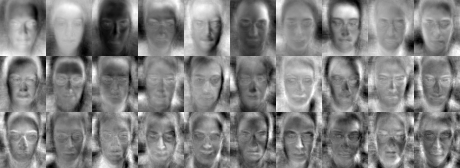
\includegraphics[width=0.4\textwidth]{../results/ex1a/eigenfaces.png}
    \caption{Eigenfaces with the 30 largest eigenvalues}
    \label{fig:eigfaces1}
\end{figure}

\begin{figure}
    \centering
    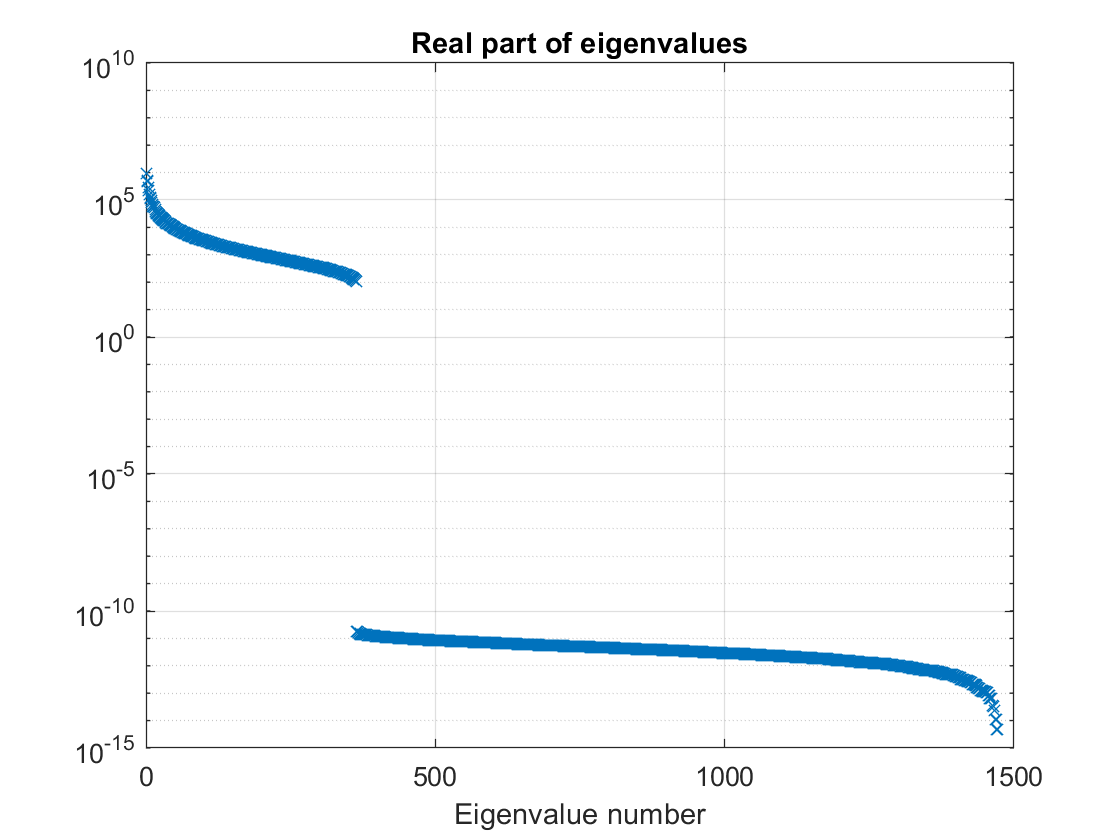
\includegraphics[width=0.4\textwidth]{../results/ex1a/eigenvalues.png}
    \caption{Real part of all PCA eigenvalues (semi-log-y axis)}
    \label{fig:eigvals1}
\end{figure}

\begin{figure}
    \centering
    
\includegraphics[width=0.1\textwidth]{../results/ex1a/mean_image.png}
    \caption{Mean image of the training dataset}
    \label{fig:mean_im1}
\end{figure}

\subsubsection{Part b)}
\begin{figure}
    \centering
    \includegraphics[width=0.5\textwidth]{../results/ex1b/eig_diff.png}
    \caption{Comparison of the high-dimensional and low-dimensional computations of eigenvalues and eigenvectors}
    \label{fig:eig_diff1}
\end{figure}




%\bibliography{IEEEabrv,./refs}
%\bibliographystyle{IEEEtran}

\end{document}